%\part{Konstruktion}
%\chapter{Programmlogik}

\section{SEARCHExtraction}
Die SearchExtraction nimmt ein WebContent-Objekt entgegen und verarbeitet es zu einem SearchModels-Objekt. Hierbei wird der HTML-Code, der im WebContent enthalten ist, auf Search-Tags abgesucht. Diese Search-Tags werden dann zu SearchModel-Objekten zusammengebaut und in einem SearchModels-Objekt gesammelt.\newline
Für den Ablauf der Analyse und Erzeugung ist der SearchManager zuständig. Die Methoden für die Analyse des HTML-Codes stellt die RegexForSEARCH zur Verfügung.

\begin{figure}[h]
	\centering
	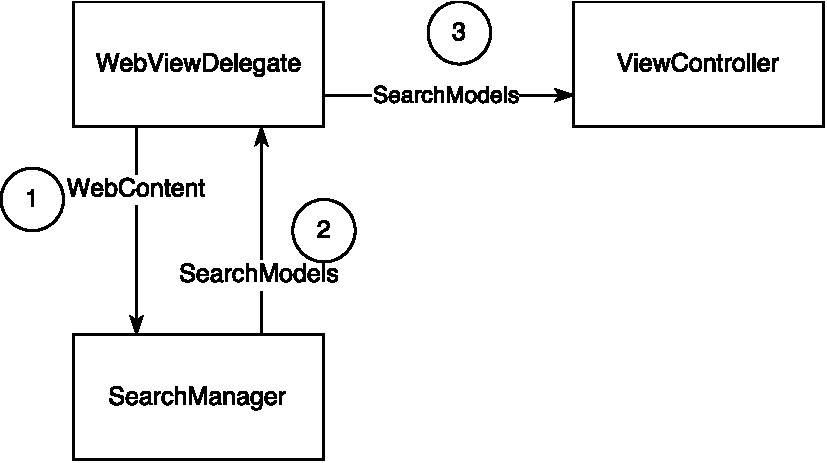
\includegraphics[width=\textwidth]{UI_WebContent_SearchModel_Usage}
	\caption{Umwandeln eines WebContent-Objekts in ein SearchModels-Objekt}
	\label{fig:WebContent zu SearchModels}
\end{figure}

Die obige Darstellung beschreibt den Ablauf und die Übergabestellen der Schnittstellen WebContent und SearchModels. Der WebContent, erzeugt vom WebViewDelegate, wird in Schritt 1 dem SearchManager übergeben. Der SearchManager erzeugt aus dem WebContent die SearchModels und gibt diese in Schritt 2 an den WebViewDelegate zurück. Der WebViewDelegate übergibt dann das SearchModels-Objekt an den ViewController, wo es zur Verfügung für die anderen Packages steht.

\subsection{SearchManager}
\subsection{RegexForSEARCH}

%\subsubsection{Unterteilabschnitt}
%\paragraph{Paragraph}
%\subparagraph{Unterparagraph}
